\begin{frame}
\frametitle{}
\begin{center}
{\fontsize{48}{55}\selectfont
{\color{title} Working\\
with\\
data\\}}
\end{center}
\end{frame}


\begin{frame}
 Read a graph stored in a file using common graph formats.
\begin{description}
\item [edge lists]
\item [adjacency lists]
\item [GML]
\item [GraphML]
\item [Pajek]
\item [LEDA]
\end{description}

\end{frame}




\begin{frame}[fragile]
\frametitle{Drawing with other programs}
\centerline{Graphviz}
\centerline{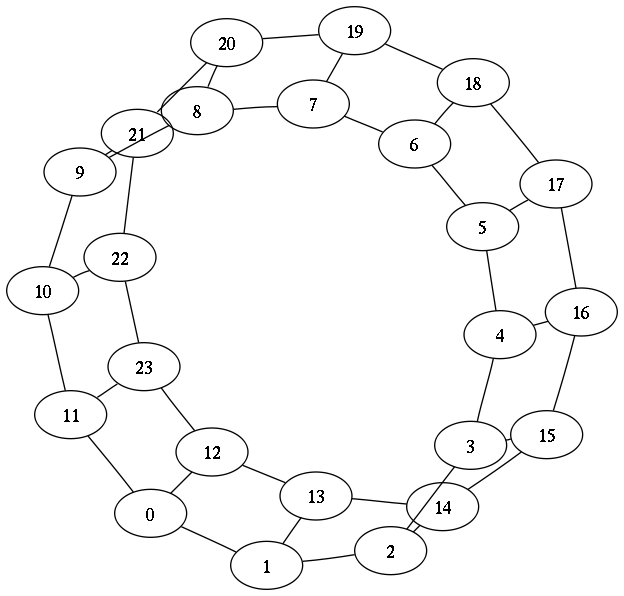
\includegraphics[width=0.5\columnwidth]{graphvizladder}}

Output to: dot, GML, LEDA, edge list, adjacency list, YAML,
sparsegraph6, GraphML

\end{frame}
